%% %%%%%%%%%%%%%%%%%%%%%%%%%%%%%%%%%%%%%%%%%%%%%%%%%
%% Template for a conference paper, prepared for the
%% Food and Resource Economics Department - IFAS
%% UNIVERSITY OF FLORIDA
%% %%%%%%%%%%%%%%%%%%%%%%%%%%%%%%%%%%%%%%%%%%%%%%%%%
%% Version 1.0 // November 2019
%% %%%%%%%%%%%%%%%%%%%%%%%%%%%%%%%%%%%%%%%%%%%%%%%%%
%% Ariel Soto-Caro
%%  - asotocaro@ufl.edu
%%  - arielsotocaro@gmail.com
%% %%%%%%%%%%%%%%%%%%%%%%%%%%%%%%%%%%%%%%%%%%%%%%%%%
\documentclass[11pt]{article}
\usepackage{UF_FRED_paper_style}

\usepackage{lipsum}  %% Package to create dummy text (comment or erase before start)

%% ===============================================
%% Setting the line spacing (3 options: only pick one)
% \doublespacing
% \singlespacing
\onehalfspacing
%% ===============================================

\setlength{\droptitle}{-5em} %% Don't touch

% %%%%%%%%%%%%%%%%%%%%%%%%%%%%%%%%%%%%%%%%%%%%%%%%%%%%%%%%%%
% SET THE TITLE
% %%%%%%%%%%%%%%%%%%%%%%%%%%%%%%%%%%%%%%%%%%%%%%%%%%%%%%%%%%

% TITLE:
\title{A Data Analysis Replication on Minimum Wages and Employment: A Case Study of the Fast-Food Industry in New Jersey and Pennsylvania
}

% AUTHORS:
\author{Jancer Wellington da Silva Gomes Filho\\% Name author
    \href{mailto:jancer.gomes@copin.ufcg.edu.br}{\texttt{jancer.gomes@copin.ufcg.edu.br}} %% Email author 1 
% \and Second Author\\% Name author
%     \href{mailto:secondauthor@ufl.edu}{\texttt{secondauthor@ufl.edu}} %% Email author 2
% \and Third Author\\% Name author
%     \href{mailto:thirdauthor@ufl.edu}{\texttt{thirdauthor@ufl.edu}}%% Email author 3
%\and Forth Author\\% Name author
%    \href{mailto:forthuthor@ufl.edu}{\texttt{forthuthor@ufl.edu}}%% Email author 4
    }
    
% DATE:
% \date{\today}
\date{July 9, 2024}

% %%%%%%%%%%%%%%%%%%%%%%%%%%%%%%%%%%%%%%%%%%%%%%%%%%%%%%%%%%
% %%%%%%%%%%%%%%%%%%%%%%%%%%%%%%%%%%%%%%%%%%%%%%%%%%%%%%%%%%
\begin{document}
% %%%%%%%%%%%%%%%%%%%%%%%%%%%%%%%%%%%%%%%%%%%%%%%%%%%%%%%%%%
% %%%%%%%%%%%%%%%%%%%%%%%%%%%%%%%%%%%%%%%%%%%%%%%%%%%%%%%%%%
% ABSTRACT
% %%%%%%%%%%%%%%%%%%%%%%%%%%%%%%%%%%%%%%%%%%%%%%%%%%%%%%%%%%
% %%%%%%%%%%%%%%%%%%%%%%%%%%%%%%%%%%%%%%%%%%%%%%%%%%%%%%%%%%
{\setstretch{.8}
\maketitle
% %%%%%%%%%%%%%%%%%%
\begin{abstract}
% CONTENT OF ABS HERE--------------------------------------

Research on empirical Social Sciences have faced the ages-long difficulty of measuring (causal) effects without conducting experiments.
This occurs because of various constraints, of both practical and ethical nature. In this work, I replicate the data analysis of "Minimum Wages and Employment: A Case Study of the Fast-Food Industry in New Jersey and Pennsylvania" by \citet{RePEc:aea:aecrev:v:84:y:1994:i:4:p:772-93}, a foundational paper in the use of DiD. It has estimated the causal impact of a law which raised the minimum wage in New Jersey from \$4.25 to \$5.05, on April 1, 1992, specially in relation to its repercussion in employment. The authors defined full-time-equivalent (FTE) employment, the outcome of interest, as "the number of full-time workers [including managers] plus 0.5 times the number of part-time workers." Consistent with the replicated paper, I found an estimated causal effect of the intervention: a raise in 2.76 (approx. 13\%) in full-time-equivalent employment per store.

% END CONTENT ABS------------------------------------------

\noindent
\textit{\textbf{Keywords: }%
differences-in-differences; mininum wage; econometrics; replication.} \\ %% <-- Keywords HERE!
% \textit{\textbf{JEL Classification: }%
% Q12; C22; D81.} %% <-- JEL code HERE!

\end{abstract}
}

% %%%%%%%%%%%%%%%%%%%%%%%%%%%%%%%%%%%%%%%%%%%%%%%%%%%%%%%%%%
% %%%%%%%%%%%%%%%%%%%%%%%%%%%%%%%%%%%%%%%%%%%%%%%%%%%%%%%%%%
% BODY OF THE DOCUMENT
% %%%%%%%%%%%%%%%%%%%%%%%%%%%%%%%%%%%%%%%%%%%%%%%%%%%%%%%%%%
% %%%%%%%%%%%%%%%%%%%%%%%%%%%%%%%%%%%%%%%%%%%%%%%%%%%%%%%%%%

% --------------------
\section{Introduction}
% --------------------
Research on empirical Social Sciences have faced the ages-long difficulty of measuring (causal) effects without conducting experiments.
This occurs because of various constraints, of both practical and ethical nature.

In the frequent absence of experiments, researchers in this field have developed many techniques to work with observational data and still be able to identify and measure causal relations between objects. With a combination of assumptions, statistical techniques and ever so increasing availability of data, we are able to confidently assess causality.

One of the most prominent and frequently used methods is Differences-in-differences (DiD), which takes advantages of so called natural experiments.

In this work, I replicate the data analysis of "Minimum Wages and Employment: A Case Study of the Fast-Food Industry in New Jersey and Pennsylvania" by \citet{RePEc:aea:aecrev:v:84:y:1994:i:4:p:772-93}, a foundational paper in the use of DiD. It has estimated the causal impact of a law which raised the minimum wage in New Jersey from \$4.25 to \$5.05, on April 1, 1992, specially in relation to its repercussion in employment. The authors defined full-time-equivalent (FTE) employment, the outcome of interest, as "the number of full-time workers [including managers] plus 0.5 times the number of part-time workers."

 Card and Krueger (henceforth, C\&K) found that the increase in minimum wage did not harm employment. In fact, fast food restaurants in NJ increased employment by 13 percent, relative to stores in PA. Such findings challenged the prevalent idea that raising the minimum wage would harm employment, backed by highly-accredited papers \citep{stigler_minimum,effect_kohen}. 
 
 It is of no surprise that the original paper has stirred the economical community quite a lot, not only at the time of its publication; in fact, it continued to make ripples for several years. In fact, on the year following its publication, \citet{neumark_1} published a working paper which used a different dataset and challenged C\&K's findings. The authors have then reexamined the matter, using a comprehensive data obtained from the Bureau of Labor Statistics's ES-202 file \citep{card_reanalysis}. The story didn't end then and there, as there was a new article by \citet{Neumark_comment}, followed by yet another reply paper \citep{card_reply}.

% --------------------
\section{Materials and Methods}
% --------------------

% \lipsum[7-9] % Dummy text. Erase before write
\subsection{Differences-in-differences}

    The replicated paper and this replication likewise make use of a statistical method called differences-in-differences, which estimates the treatment effect on treated units by comparing their changes over time to those of untreated ("control") units: subjects whose characteristics are comparable/equivalent to the treated group's, except for exposure status.

    It relies on the key assumption that, under no treatment, the outcome of interest varies the same way for both treated and control units; this is often referred to as the "parallel trends" assumption. Since the treated group is at first expected to show a trend similar to that of control unit, deviations from that trend are accounted for as the causal impact of the treatment.

\subsection{Data Source and Analysis}

    The dataset analysed in this paper comes from the survey conducted by the authors of the original paper. It was collected mostly via telephone calls to the stores in the sample. The  stores in question are in Pennsylvania and New Jersey, specially in the areas close to the border between the two states.

    Data were collected in two rounds: one in February 1992, and another in November 1992, after the raise in New Jersey's minimum wage came into effect.

    Analyses were conducted using R 4.4.1 \citep{R_lang}, especially the statistical analysis ecosystem named Tidyverse \citep{Tidyverse}. A R Markdown with the main scripts used in the making of this work are available on our associated GitHub repository.




% --------------------
\section{Results}
% --------------------
I was able to reproduce the main columns from Table 3 of the original paper (indexed here as Table 1), displaying the FTE employment in both Pennsylvania and New Jersey.

Row 3 displays the main finding of the study, comparing the change in mean FTE employment between the two states.

\begin{table}[H]
\centering
\renewcommand{\arraystretch}{1.2}
\begin{tabular}{|lp{6cm}|l|l|l|}
  \hline
 & Variable & Pennsylvania & New Jersey & Difference \\ 
  \hline
1. & FTE employment before,\newline all available observations & 23.33 & 20.44 & -2.89 \\ 
  2. & FTE employment after, \newline all available observations & 21.17 & 21.03 & -0.14 \\ 
  3. & Change in mean FTE employment & -2.17 & 0.59 & 2.76 \\ 
  4. & Change in mean FTE employment, balanced sample of stores & -2.28 & 0.47 & 2.75 \\ 
  5. & Change in mean FTE employment, setting FTE at temporarily closed stores to 0 & -2.28 & 0.23 & 2.51 \\ 
   \hline
\end{tabular}
\captionsetup{justification=centering}
\caption{Average Employment per Store Before and After the Rise in New Jersey Minimum Wage} 
\label{tab:indCC}
\end{table}


The plot below shows the expected mean FTE employment outcome in New Jersey, under the assumption of parallel trends and no effect (18.27), compared to the actual outcome (21.03). The difference between those values is the estimated causal effect of the intervention: a raise in 2.76 (approx. 13\%) in full-time-equivalent employment per store. 


\begin{figure}[H]
    \centering
        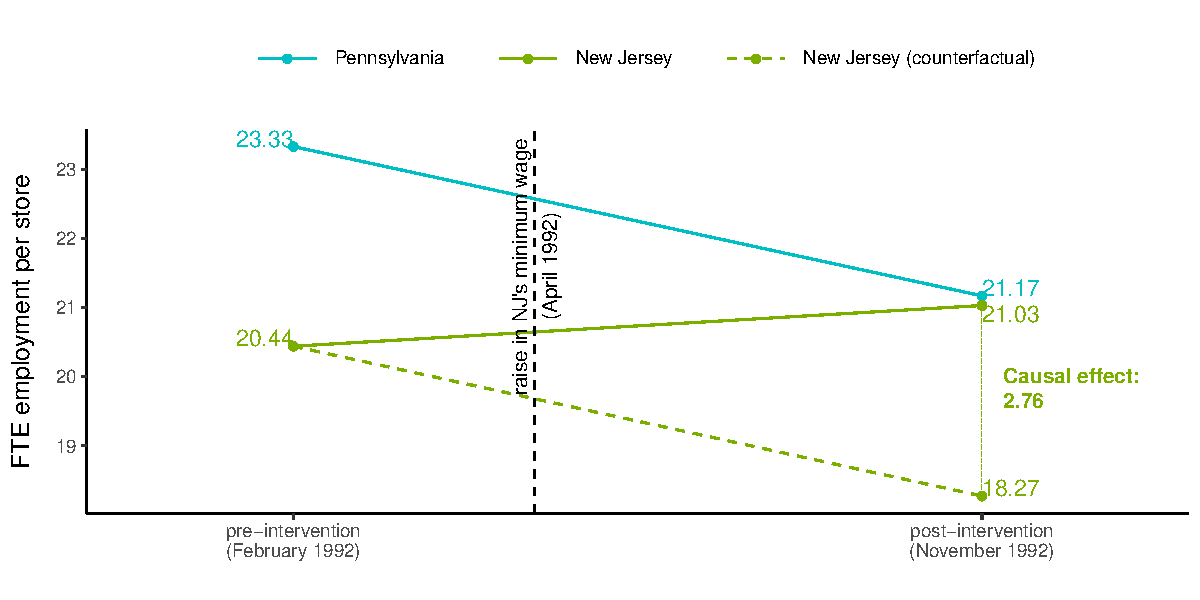
\includegraphics[scale=.6]{figures/fte_did.pdf}
    \caption{DID visualization of the impact of minimum wage raise on FTE employment.}
    \label{fig:1}
\end{figure}

The results found in this work are consistent with the original paper's.

% \lipsum[12-13] % Dummy text. Erase before write

% --------------------
\section{Discussion and Conclusions}
% --------------------

This paper has assessed the changes in full-time-equivalent employment in restaurants located in the states of Pennsylvania and New Jersey. This work has validated part of the data analyses found in the original paper by \citet{RePEc:aea:aecrev:v:84:y:1994:i:4:p:772-93}. I found no bad practices in the statistical assessment done by the authors, and the results displayed here are consistent with the source report.

Evidence in the direction that raising the minimum wage does not result in unemployment (at least in fast-food restaurants, with high concentration of minimum-wage workers) has an important meaning for policymakers. Changes in the minimum-wage have a substantial impact in the economy and in the lives of working-class people. Understanding if and how much of a raise is most beneficial requires evidence regarding its multiple impacts.

In future studies, it is important to address limitations of a simple, canonical DiD model, and also to address the effect of raising the minimum-wage in various economical and geographical settings.



\medskip

\bibliography{references.bib} 

\newpage

% %%%%%%%%%%%%%%%%%%%%%%%%%%%%%%%%%%%%%%%%%%%%%%%%%%%%%%%%%%
% %%%%%%%%%%%%%%%%%%%%%%%%%%%%%%%%%%%%%%%%%%%%%%%%%%%%%%%%%%
% TABLES
% %%%%%%%%%%%%%%%%%%%%%%%%%%%%%%%%%%%%%%%%%%%%%%%%%%%%%%%%%%
% %%%%%%%%%%%%%%%%%%%%%%%%%%%%%%%%%%%%%%%%%%%%%%%%%%%%%%%%%%



% %%%%%%%%%%%%%%%%%%%%%%%%%%%%%%%%%%%%%%%%%%%%%%%%%%%%%%%%%%
% %%%%%%%%%%%%%%%%%%%%%%%%%%%%%%%%%%%%%%%%%%%%%%%%%%%%%%%%%%
% FIGURES
% %%%%%%%%%%%%%%%%%%%%%%%%%%%%%%%%%%%%%%%%%%%%%%%%%%%%%%%%%%
% %%%%%%%%%%%%%%%%%%%%%%%%%%%%%%%%%%%%%%%%%%%%%%%%%%%%%%%%%%



% ==========================
% ==========================
% ==========================


\end{document}